% Chapter: On the Recoverability of Coalescence Phase and Polarization Angle
% from Gravitational-Wave Strain: A Systematically Verified Null Result
% Under the Corrected Combination Formula
%
% Requires (thesis preamble): amsmath, amssymb, booktabs, graphicx
% Figures are referenced from the experiment directory; adjust \graphicspath
% or copy the PNGs into the thesis figures/ directory.
%
% Draft status: chapter number, cross-references, and \cite keys are
% placeholders to be resolved against the thesis bibliography. All
% quantitative values are taken verbatim from the redo's experiment record on
% branch poc/phic-psi-degeneracy-redo (see the claim-to-artifact map in the
% chapter appendix).
%
% RELATIONSHIP TO THE PRIOR CHAPTER.
% An earlier version of this investigation (experiments/phic_psi_poc/,
% branch poc/phic-psi-degeneracy, preserved on archive/phic-psi-poc-v1)
% reached the same null conclusion using a combination formula, phi_c +- 2psi,
% that a reviewer later showed to be physically wrong: this dataset's
% injection convention makes phi_c enter the strain doubled too, so the
% correct combination is 2phi_c +- 2psi. This chapter is a full redo under
% the corrected formula, not an edit of the original, and is written to
% stand on its own. Two internal documents back every comparative claim and
% are cited directly rather than re-derived:
% experiments/phic_psi_poc-redo/original_vs_redo_comparison.md (every number
% from both investigations, side by side) and
% experiments/phic_psi_poc-redo/review_inheritance_map.md (every concern
% raised by the prior chapter's three adversarial reviewers, checked against
% this redo's actual artifacts). The redo's evidentiary architecture differs
% from the prior chapter's in one load-bearing way, disclosed in Sec 1
% rather than left for the reader to discover in the Results: the prior
% chapter certified its null on two models that passed a pre-registered
% metric-health gate; in this redo, that gate never passed, at any
% regularization strength tried, for either combination vector, in either
% training mode. The null defended below rests on a broad, convergent
% battery of checks run across all four down-selected models instead.
%
% This chapter has NOT yet been through adversarial AI review (unlike the
% prior chapter's four rounds). See review_inheritance_map.md for which of
% the prior chapter's review concerns already transfer by construction, which
% are genuinely new and need a fresh targeted review of the evidentiary
% architecture specifically, and which are concrete physics/ablation gaps
% (synthetic poc_b ablation, high-SNR/Fisher check, dataset regeneration,
% ridge test) re-affirmed here as still open in Sec 8.5 rather than silently
% dropped a second time.

\usepackage{geometry}
\usepackage{graphicx}
\usepackage{amssymb}
\usepackage{amsfonts}
\usepackage{booktabs}
\usepackage{amsopn}
\usepackage{amsmath}
\usepackage{amstext}

\graphicspath{{../}{../diagnostic_output/}{../analysis_output/}{../bootstrap_output/}{../snr_output/}{../inclination_output/}{../perturbation_trace_output/}{../rose_plot_output/}{../sky_mollweide_output/}}


\chapter{On the Recoverability of Coalescence Phase and Polarization Angle from Gravitational-Wave Strain: A Systematically Verified Null Result Under the Corrected Combination Formula}
\label{ch:phic-psi-degeneracy-redo}


\section{Introduction}
\label{sec:phicpsi:intro}

Deep-learning approaches to gravitational-wave parameter estimation have matured rapidly, from early proof-of-concept classifiers~\cite{george2018deep} to amortized neural posterior estimators that approach the accuracy of stochastic-sampling pipelines~\cite{gabbard2022vitamin,dax2021dingo} at a fraction of their latency.
Most of this progress has concentrated on parameters that imprint strongly and non-degenerately on the observed strain: the chirp mass through the phase evolution~\cite{cutler1994gw}, the merger time through the temporal localization of the signal, the signal-to-noise ratio through overall amplitude, and the sky position through inter-detector time delays and antenna-pattern amplitudes.

Two extrinsic parameters have received far less attention as direct regression targets: the orbital phase at coalescence, $\varphi_c$, and the polarization angle, $\psi$.
For the dominant quadrupole ($\ell=2$, $|m|=2$) mode of a quasi-circular compact binary, the two polarization states are
\begin{equation}
    h_+ \propto (1+\cos^2\iota)\,\cos\!\bigl(2\varphi(t)+2\varphi_c\bigr),
    \qquad
    h_\times \propto 2\cos\iota\,\sin\!\bigl(2\varphi(t)+2\varphi_c\bigr),
\end{equation}
and the detector response mixes them through antenna patterns that depend on $2\psi$~\cite{cutler1994gw,sathyaprakash2009physics}.
Both $\varphi_c$ and $\psi$ enter the strain doubled, so the analytically degenerate combination in the face-on limit is $\mathbf{2\varphi_c \pm 2\psi}$, with the sign set by the sign of $\cos\iota$.
The correction traces directly to how \texttt{coa\_phase} is injected in this dataset's generator: it is PyCBC/LALSimulation's orbital reference phase, and for a dominant-mode-only waveform that orbital phase enters the strain through $e^{i\cdot 2\cdot\text{coa\_phase}}$, exactly like $\psi$ already does.
In the face-on limit ($\cos\iota \to \pm 1$) the signal becomes circularly polarized and depends on $\varphi_c$ and $\psi$ only through this single combination, so the individual angles are exactly unidentifiable there, and only partially disentangled as the inclination moves toward edge-on.
Bayesian samplers absorb this structure into broad, multimodal joint posteriors~\cite{veitch2015lalinference}; a point-estimate regression network has no such refuge.

This chapter asks:
\begin{quote}
\itshape Can $\varphi_c$ and $\psi$ be recovered from strain alone by a deep neural network --- individually, or through their better-conditioned sum/difference combinations --- or is the degeneracy effectively exact for a realistic detection-scale population?
\end{quote}

The answer is a \textbf{null result}: across four down-selected architectures, two head parameterizations, three values of the magnitude-regularization coefficient, and a comprehensive diagnostic battery, no model performed measurably better than random guessing on either angle, while the same networks simultaneously recovered chirp mass, merger time, signal-to-noise ratio, and sky position with high fidelity from the same shared features.
No model here ever cleared the pre-registered metric-health gate that would have certified it as a clean test.
The null defended here instead rests on convergence across four independent lines of evidence --- direct inspection of the prediction distributions, a code-level gradient-health trace ruling out an implementation bug, a formal label-permutation bootstrap, and population stratification by inclination and signal-to-noise ratio --- applied uniformly to all four down-selected models, without excluding any on interpretability grounds.
This study additionally surfaced two findings: a genuine, SNR-monotonic partial sky-localization skill in one architecture (\texttt{cnn\_attention}), unrelated to the $\varphi_c/\psi$ question, and a small but statistically real sub-floor signal in the inclination control head, which had been assumed to be clean noise.

The chapter is organized as follows, with one section deliberately compressed.
Section~\ref{sec:phicpsi:problem} formalizes the problem and the circular-regression framework.
Section~\ref{sec:phicpsi:prereq} presents the analytic prerequisite study.
Section~\ref{sec:phicpsi:methods} details the datasets, architectures, losses, and training protocol, including the combination construction.
Section~\ref{sec:phicpsi:arc} summarizes, briefly, two optimization pathologies in this training pipeline (tanh saturation, magnitude drift) and how they were fixed prior to the main sweep.
Section~\ref{sec:phicpsi:results} presents the defended null result, its verification battery, and the two new findings.
Section~\ref{sec:phicpsi:prereg} describes the pre-registered magnitude-penalty retune and its outcome.
Section~\ref{sec:phicpsi:discussion} discusses interpretation, limitations, and future work; Section~\ref{sec:phicpsi:conclusion} concludes.


\section{Problem Formulation}
\label{sec:phicpsi:problem}

\subsection{Targets and the degeneracy hypothesis}
\label{sec:phicpsi:targets}

We consider a ten-parameter description of a compact binary coalescence signal injected into two-detector noise: chirp mass $\mathcal{M}$, mass ratio $q$, inclination $\iota$, coalescence phase $\varphi_c$, polarization angle $\psi$, declination, right ascension, injection time, merger time within the analysis window, and network signal-to-noise ratio.
Seven of these are used as supervised regression targets (mass ratio and injection time are excluded; \S\ref{sec:phicpsi:dataset}).
The scientific targets are $\varphi_c \in [0, 2\pi)$, period $2\pi$, and $\psi \in [0, \pi)$, period $\pi$.
Inclination, chirp mass, merger time, SNR, and sky position are retained as \emph{control heads}: parameters trained through the identical pipeline whose success or failure calibrates what the network can extract from strain when information is present.

The \textbf{degeneracy hypothesis} under test is: \emph{$\varphi_c$ and $\psi$ carry no strain-only recoverable signal for this population, in this architecture and loss family} --- a point-estimating network can do no better than the optimal constant prediction, because for most of the population the likelihood constrains only the combination $2\varphi_c \pm 2\psi$, and the remaining direction is unconstrained.
The alternative hypothesis motivating the experimental design is that even if $\varphi_c$ and $\psi$ are individually unrecoverable, their \textbf{sum and difference combinations} may be well-conditioned: a network parameterized in $2\varphi_c \pm 2\psi$ combination space, with a curriculum that weights each combination according to how well the current inclination constrains it, might learn the recoverable structure that a naive per-angle parameterization misses.

Conditioning on inclination $\iota$ --- tested as future work in \S\ref{sec:phicpsi:future} --- is treated throughout as a \emph{training-paradigm design choice}, motivated by the analytic structure of \S\ref{sec:phicpsi:prereq} showing that the well-constrained combination is recoverable given $\iota$, not as a forced move necessitated by a proof that $\iota$ itself is unrecoverable; \S\ref{sec:phicpsi:inclination} shows $\iota$ in fact carries a small, real signal, which sharpens rather than resolves this question.
No model in this chapter takes $\iota$, or any function of it, as an input at any stage; it appears only as a control \emph{output} head.

\subsection{Circular regression framework}
\label{sec:phicpsi:circular}

Periodic targets are regressed on the unit circle~\cite{mardia2000circular}.
An angle $\theta$ with period $T$ is encoded as the two-vector $\mathbf{u}(\theta) = (\sin(2\pi\theta/T), \cos(2\pi\theta/T))$, so the $\psi$ head, with $T=\pi$, physically encodes $2\psi$.
Each periodic head outputs a raw two-vector $\mathbf{v}\in\mathbb{R}^2$, projected onto the unit circle by \texttt{tf\_normalize\_unit}, $\hat{\mathbf{u}} = \mathbf{v}/\sqrt{\max(\|\mathbf{v}\|^2,\varepsilon)}$ --- a clamp on the squared norm, for a stable gradient at $\mathbf{v}=\mathbf{0}$, rather than a floor on $\|\mathbf{v}\|$ itself --- and trained with the cosine (circular) loss $L_{\text{circ}} = 1 - \cos\Delta\theta$.
For uniformly distributed targets and any fixed prediction, the expected circular loss is exactly 1; the null baselines are $\text{ang\_MAE} = \pi/2 \approx 1.5708$~rad for $\varphi_c$ and $\iota$, $\pi/4 \approx 0.7854$~rad for $\psi$.
Two further diagnostic statistics recur throughout: the circular resultant $\text{circ}_r = \|\text{mean}(\hat{\mathbf{u}})\|$, which measures mode collapse ($\text{circ}_r \to 1$ means all predictions concentrate at one angle), and $\text{std\_ratio}$, the ratio of the standard deviation of a head's raw outputs to that of the encoded targets, a monitor of raw-magnitude health with a healthy band of $[0.5, 2.0]$.
Non-periodic heads use a Huber loss on transformed targets, and the sky-position head uses a closed-form von Mises--Fisher negative log-likelihood on the unit sphere.
The inclination head keeps an architecturally distinct path --- periodic two-vector encoding, but a Huber loss on the raw output, with no \texttt{tf\_normalize\_unit} projection and no circular loss anywhere in its path.


\section{Analytic Prerequisite Study}
\label{sec:phicpsi:prereq}

The combination-space hypothesis was tested analytically, using a toy detector-response model in which \texttt{h\_plus}/\texttt{h\_cross} add $2\varphi_c$ to the orbital-phase term $2\Phi$, not $\varphi_c$ singly (\texttt{formulae\_reference.md} \S A.5).
A required self-check --- sweeping $\psi$ at fixed $2\varphi_c + 2\psi$, confirming $(R,\delta)$ stays exactly constant at $\iota=0$ --- passed to machine precision ($\max\,\text{std}(R) = 1.16\times10^{-14}$, $\max\,\text{std}(\delta) = 5.87\times10^{-16}$; \texttt{prereq\_checks\_20260914\_160834.log}), gating trust in everything that follows.

The 100-point inclination sweep (50 points per sign of $\cos\iota$, 200 sky positions, 5{,}000-draw bootstrap) confirms the expected combination structure:
\begin{itemize}
\item for $\cos\iota > 0$, combo \textbf{B} ($2\varphi_c - 2\psi$) is the better-constrained combination throughout; for $\cos\iota < 0$, combo \textbf{A} ($2\varphi_c + 2\psi$) wins --- a clean sign flip driven by the sign of $\cos\iota$;
\item the preference ratio is strongest face-on, $\approx 1.62$--$1.65\times$, decaying monotonically toward $\approx 1.04$--$1.07\times$ at edge-on, never crossing 1.0;
\item population-bootstrapped mean ratios are $1.17\times$ (95\% CI $[1.11, 1.24]$) for $\cos\iota > 0$ and $1.19\times$ (95\% CI $[1.12, 1.26]$) for $\cos\iota < 0$, with the simple two-point reference check clearing statistical significance directly.
\end{itemize}

The curriculum weight derivation (\texttt{formulae\_reference.md} \S A.7) gives $w(\text{face-on}) = 0.0000$ and $w(\text{edge-on}) = 0.1416$, with an intermediate-peak shape; training uses the analytically motivated fallback $w(\iota) = 1 - \cos^2\iota = \sin^2\iota$ rather than the fitted empirical curve.
Population balance: 28.7\% face-on ($|\cos\iota| > 0.9$), 32.7\% edge-on ($|\cos\iota| < 0.5$).

\begin{figure}[tbp]
    \centering
    
\includegraphics[width=\textwidth]{sweep_1_1_ratio_vs_iota.png}
    \caption[Analytic check of the corrected $2\varphi_c$--$2\psi$ degeneracy structure]{Analytic check of the corrected $2\varphi_c$--$2\psi$ degeneracy structure, ratio of the strain correlation with the well-constrained combination to the poorly-constrained one, as a function of inclination.}
    \label{fig:phicpsi:redo:sweep}
\end{figure}

The prerequisite study's verdict is GO: the combination structure exists in the data, with the predicted sign behavior.
Whatever the networks below fail to learn, they do not fail for want of an analytically real target.


\section{Methods}
\label{sec:phicpsi:methods}

\subsection{Dataset}
\label{sec:phicpsi:dataset}

All experiments use a single pre-generated dataset, \texttt{combined\_repackaged.hdf} (referenced by \texttt{config\_baseline.yaml}): 25{,}000 training and 5{,}000 validation samples, two-detector (H1/L1), network SNR uniform in $[7,15]$.
The injection convention behind the combination formula of \S\ref{sec:phicpsi:intro} is traced directly through the dataset's actual generator source code (\texttt{ml-gw-search/mlgwsc-1/gen.py:202}, \texttt{ml-gw-search/extended\_mass/gen.py:179}), confirming PyCBC/LALSimulation's \texttt{phiRef} convention and IMRPhenomD, dominant-mode-only, from code rather than recollection; the dataset itself was not regenerated from a version-controlled generator, so a reproducibility gap remains open (\S\ref{sec:phicpsi:threats}, \S\ref{sec:phicpsi:future}).

\subsection{Trunk architectures}
\label{sec:phicpsi:trunks}

Five one-dimensional trunk architectures (\texttt{tcn}, \texttt{cnn\_baseline}, \texttt{cnn\_attention}, \texttt{inception\_time}, \texttt{resnet1d}) were evaluated, all mapping the $(4096,2)$ input to a pooled feature vector shared by every head.
\texttt{mode: baseline} and \texttt{mode: poc} on the primary \texttt{tcn} trunk give the named configurations \texttt{poc\_a} and \texttt{poc\_b}.

\subsection{Head parameterizations}
\label{sec:phicpsi:heads}

\textbf{Baseline mode} uses independent circular-loss heads directly on $\varphi_c$ and $\psi$.
\textbf{PoC mode} (\texttt{SumDiffTrainer}) constructs the two combination heads explicitly rather than treating $\varphi_c$ and $\psi$ as independent outputs.
The $\varphi_c$ head's unit vector, $\mathbf{z}_{\varphi_c}$, is first passed through a \texttt{double\_angle} operation, $\mathbf{z}_{2\varphi_c} = \text{complex\_mul}(\mathbf{z}_{\varphi_c}, \mathbf{z}_{\varphi_c})$, which turns a unit vector at angle $\varphi_c$ into one at angle $2\varphi_c$ (\texttt{formulae\_reference.md} \S A.1.5); the $\psi$ head's own encoding already stores $2\psi$ internally, since \texttt{polarization\_angle} is declared with period $\pi$ and \texttt{PERIODIC.transform\_head} rescales by $2\pi/\text{period}$ before taking sin/cos.
The two combination vectors are then $\mathbf{z}_A = \text{complex\_mul}(\mathbf{z}_{2\varphi_c}, \mathbf{z}_\psi)$, angle $2\varphi_c + 2\psi$, and $\mathbf{z}_B = \text{complex\_mul\_conj}(\mathbf{z}_{2\varphi_c}, \mathbf{z}_\psi)$, angle $2\varphi_c - 2\psi$ (\texttt{formulae\_reference.md} \S A.2).
The isotropic circular loss, the sign-dependent per-sample curriculum weighting, and the uncertainty-weighting scheme are fixed pipeline components, applied identically to every head.
The well-constrained combination assignment ($\text{combo}_B$ for $\cos\iota\geq0$) is derived from this study's own prerequisite analysis (\S\ref{sec:phicpsi:prereq}).

\subsection{Magnitude penalty}
\label{sec:phicpsi:penalty}

Following the diagnosis in \S\ref{sec:phicpsi:arc}, all configurations add an explicit radial regularizer on the raw, pre-normalization periodic outputs, $L_{\text{mag}} = \lambda \cdot \sum \text{mean}\bigl[(\|v\|-1)^2\bigr]$, present in every configuration from the first training run.
$\lambda = 0.01$ for the Round-1 sweep (\S\ref{sec:phicpsi:results}), retuned to 0.05 and 0.10 in \S\ref{sec:phicpsi:prereg}.

\subsection{Training protocol}
\label{sec:phicpsi:protocol}

Adam, initial learning rate $10^{-3}$, \texttt{ReduceLROnPlateau} (factor 0.5, patience 5), batch size 128, 80 epochs, seed 42, uncertainty weighting with log-variance clamp $\pm 3$, Huber $\delta=1$.
Periodic epoch-10 checkpoints (\texttt{checkpoint\_every\_n: 10}) were saved throughout, not only best/final weights, per this repository's standing convention requirement.

\subsection{Evaluation}
\label{sec:phicpsi:evaluation}

Point predictions are scored by wrap-aware angular MAE, $\text{circ}_r$, and, for scalar heads, MAE/R\textsuperscript{2}.
Statistical significance is assessed by a label-permutation bootstrap ($N=10{,}000$ shuffles), and population heterogeneity is probed by SNR-tercile stratification.
Two additional checks were added in response to a genuine new finding for one architecture (\S\ref{sec:phicpsi:sky}) rather than planned in advance: a formal shuffle-null bootstrap and SNR-tercile stratification for the sky-position head's own angular separation (\texttt{bootstrap\_sky\_separation.py}, \texttt{snr\_stratification\_sky\_position.py}).


\section{Inherited Diagnostic History and Present-Day Machinery Check}
\label{sec:phicpsi:arc}

\subsection{What was inherited, not rediscovered}
\label{sec:phicpsi:inherited}

Before any measurement of the degeneracy could be trusted, two genuine optimization pathologies in this training pipeline had to be found and fixed: tanh saturation at random initialization on the periodic head output layers (fixed by switching to a linear output activation, since \texttt{tf\_normalize\_unit} already projects onto the unit circle), and, once that was fixed, a second pathology in which the isotropic circular loss provides no restoring force on the raw output's magnitude, so \texttt{tf\_normalize\_unit}'s backward pass --- which divides by that magnitude --- either crushes or explodes the angular gradient as the magnitude drifts (fixed by the explicit magnitude penalty of \S\ref{sec:phicpsi:penalty}).
Both are established facts about \emph{this codebase's training mechanism}, fixed before the Round-1 sweep in \S\ref{sec:phicpsi:results} began; the sections that follow do not re-narrate the bug hunt that found them.

\subsection{Verification on trained checkpoints}
\label{sec:phicpsi:verification}

Confirming, on the Round-1 ($\lambda=0.01$) checkpoints, that the machinery above is healthy is a prerequisite to trusting anything it produces.

\textbf{Labels are clean.}
True $\varphi_c/\psi/\iota/$right-ascension are uniform to circular resultant $\leq 0.013$.

\textbf{Gradients reach the periodic-head weights, end to end, through the corrected construction.}
A full forward/backward trace on \texttt{poc\_redo\_b}'s real trained checkpoint shows healthy, non-vanishing gradient at every stage of the combination pipeline: $dL/d(\text{combo\_A\_pred}) = 0.4245$, dropping through the new \texttt{double\_angle} stage ($dL/d(\mathbf{z}_{2\varphi_c,\text{norm}}) = 0.375$) to $dL/d(\mathbf{z}_{\varphi_c,\text{raw}}) = 0.570$ and $dL/d(\mathbf{z}_{\psi,\text{raw}}) = 0.514$ --- all comparable in order of magnitude to the healthy inclination-head baseline, 0.728 (\texttt{diagnostic\_output/diagnostic\_checks\_20260916\_113913.log}, lines 297--304).
Prediction perturbation after one optimizer step shows the periodic heads moving far more than the converged scalar control ($\text{coa\_phase}$ mean$|\Delta| = 1.61\times10^{-2}$, $\text{polarization\_angle}$ $1.33\times10^{-2}$, against mchirp's $3.28\times10^{-4}$), confirming the gradient path is live, not disconnected.

\textbf{Positive controls recover well} (Fig.~\ref{fig:phicpsi:redo:controls}): chirp mass R\textsuperscript{2} $= 0.920$--$0.960$ (\texttt{poc\_a} 0.958, \texttt{poc\_b} 0.958, \texttt{tcn} 0.960, \texttt{cnn\_attention} 0.920), merger time R\textsuperscript{2} $= 0.906$--$0.928$, SNR R\textsuperscript{2} $= 0.741$--$0.789$, sky position $4.4^\circ$--$10.3^\circ$ mean angular error.
Inclination is deliberately excluded from this positive-control list for a documented, code-level reason --- its Huber-loss, non-normalized path is architecturally distinct from $\varphi_c/\psi$'s --- not omitted quietly; its own, more nuanced result is presented on its own terms in \S\ref{sec:phicpsi:inclination}.

\begin{figure}[tbp]
    \centering
    \includegraphics[width=0.9\textwidth]{true_label_distributions.png}
    \caption{True label distributions (Check 1).}
    \label{fig:phicpsi:redo:labels}
\end{figure}

\begin{figure}[tbp]
    \centering
    \includegraphics[width=0.9\textwidth]{combo_loss_trajectories.png}
    \caption{Combo/circular-loss trajectories for \texttt{poc\_redo\_b}, all 80 epochs.}
    \label{fig:phicpsi:redo:comboloss}
\end{figure}

\begin{figure}[tbp]
    \centering
    \includegraphics[width=0.9\textwidth]{logvar_trajectories.png}
    \caption{Uncertainty-weighting $\exp(-s)$ trajectories per head.}
    \label{fig:phicpsi:redo:logvar}
\end{figure}

\begin{figure}[tbp]
    \centering
    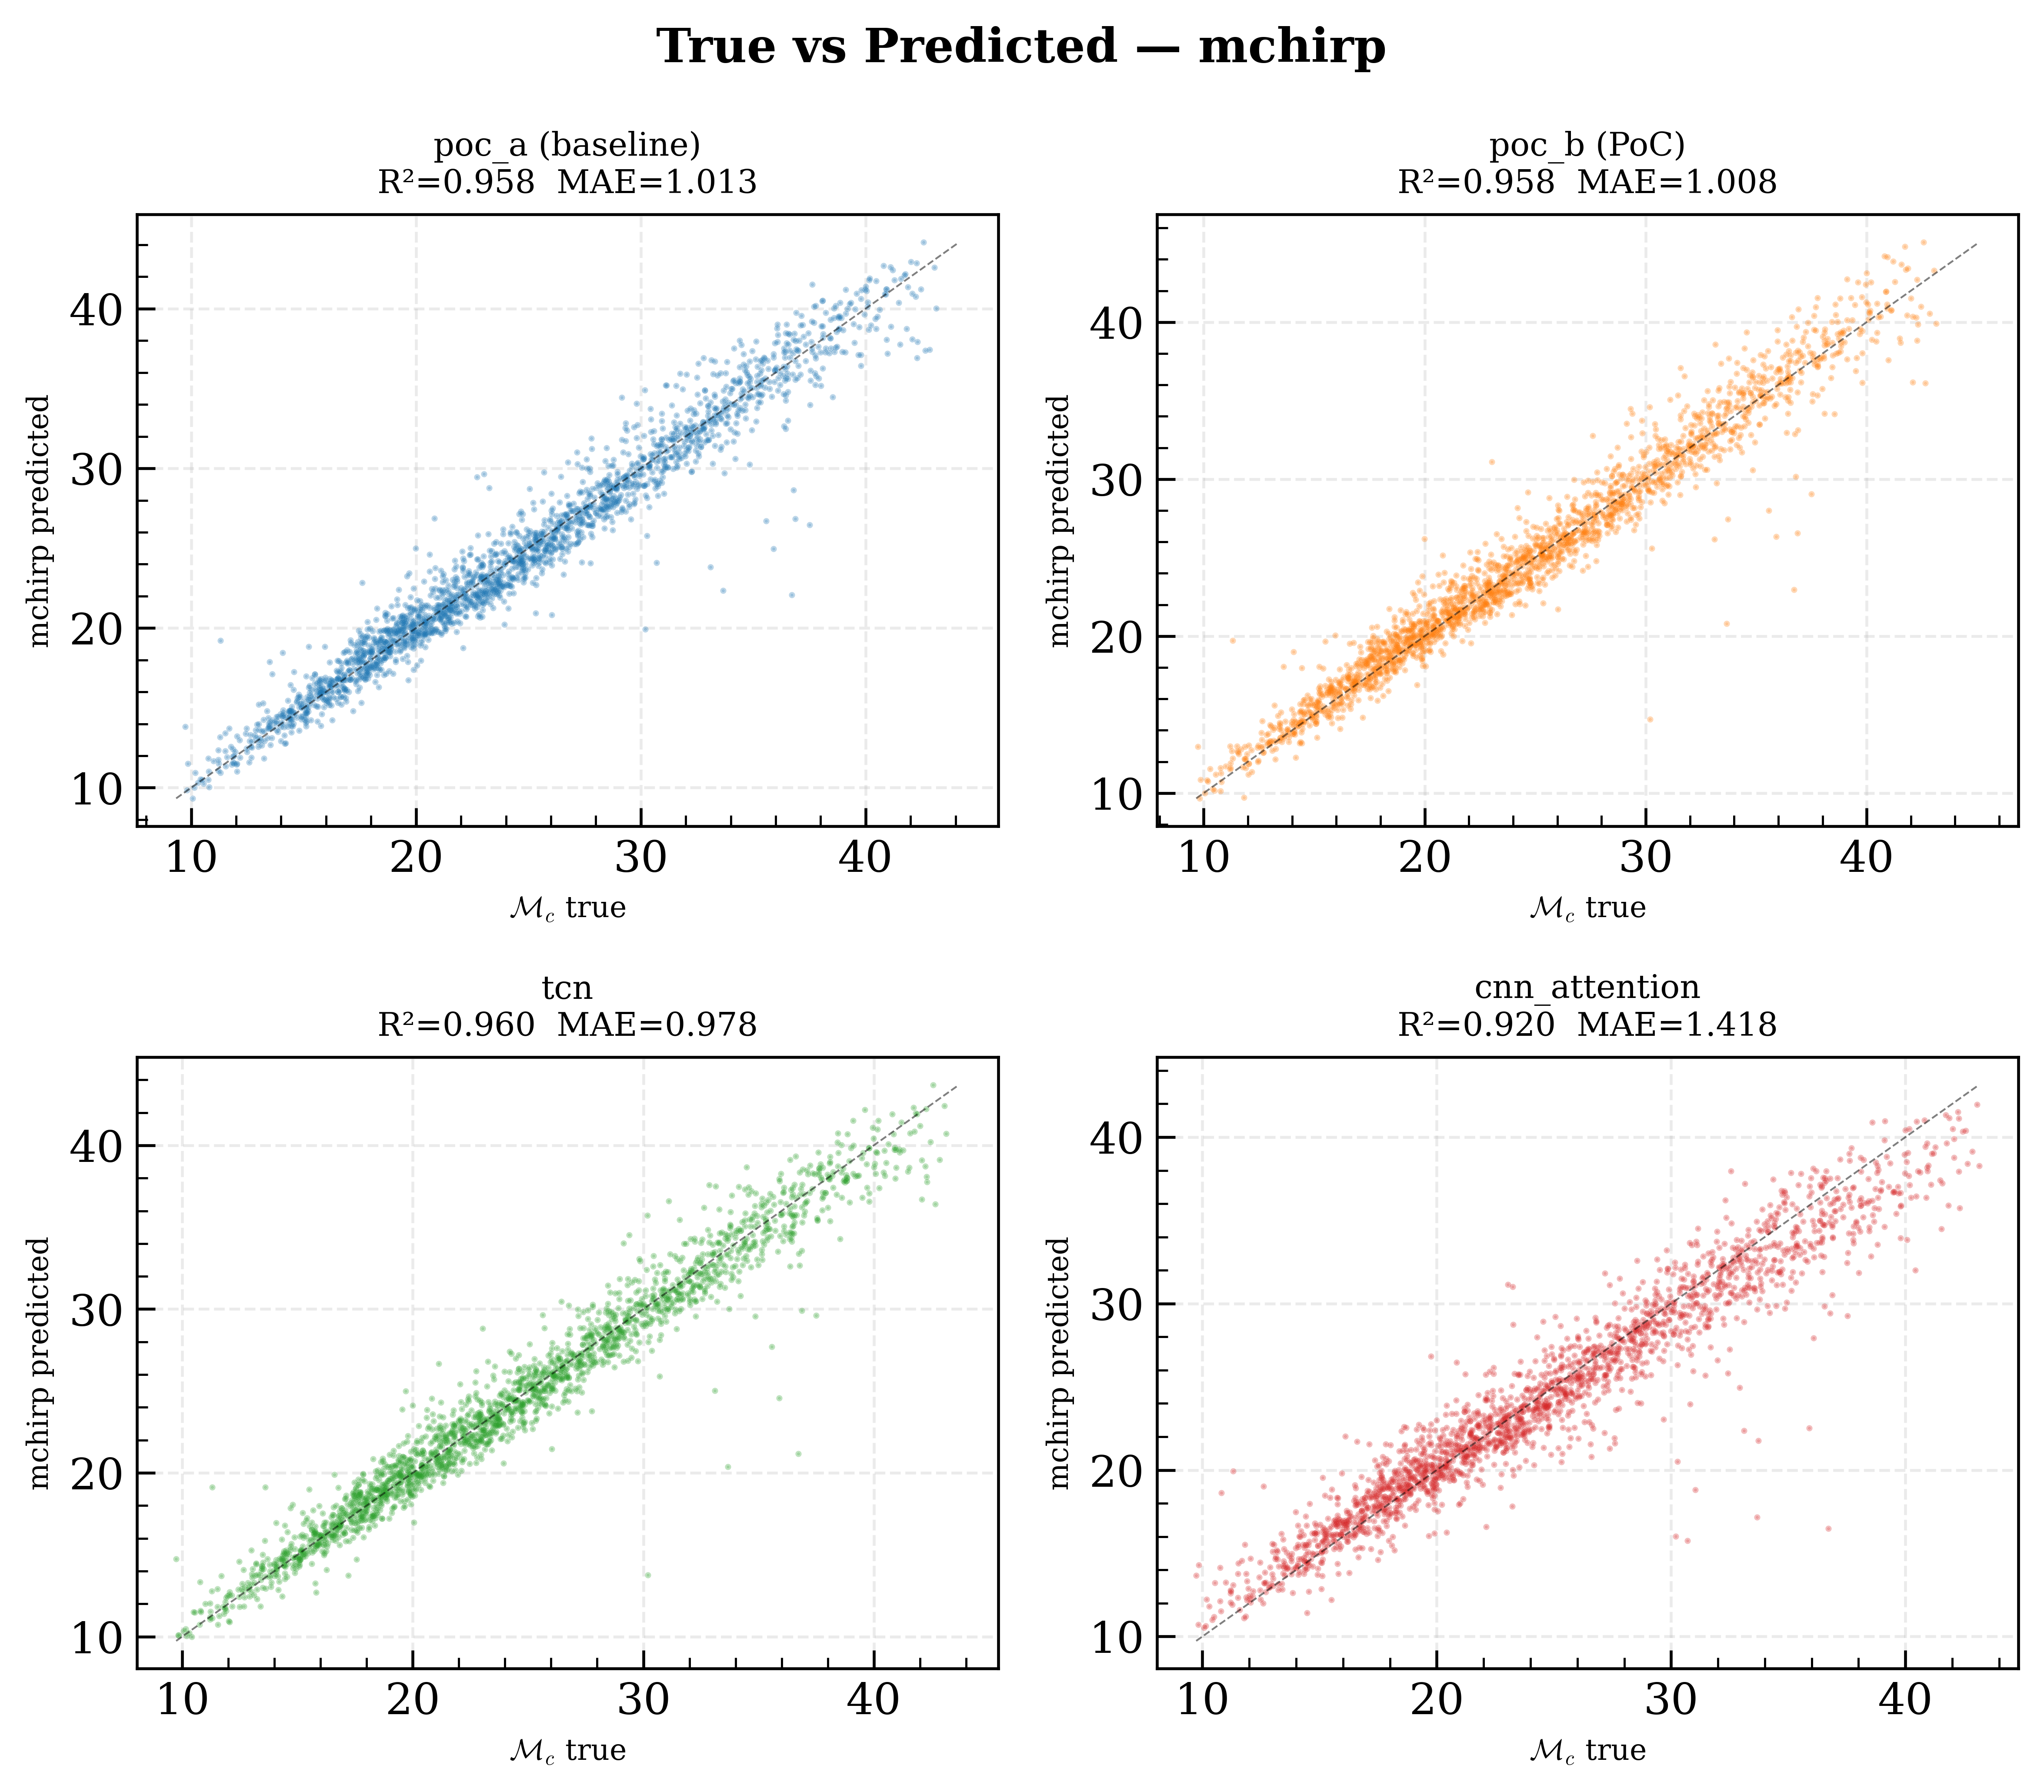
\includegraphics[width=\textwidth]{scatter_mchirp_20260916_113847.png}
    \caption{Positive-control recovery (chirp mass) for the four Round-1 models.}
    \label{fig:phicpsi:redo:controls}
\end{figure}

The machinery this study depends on is verifiably healthy.
What it produces on the actual question of interest is presented next.


\section{Results: A Defended Null, Under the Corrected Formula}
\label{sec:phicpsi:results}

\subsection{Headline result}
\label{sec:phicpsi:headline}

At epoch~79 (last-10-epoch mean), \texttt{poc\_redo\_b}'s combination-space circular loss reads combo\_A $=0.9999$, combo\_B $=0.9895$ --- both essentially at the ceiling value of 1 expected under random guessing.

\begin{table}[tbp]
    \centering
    \caption{Periodic-head recovery, four down-selected models, $\lambda=0.01$, Round~1 (2026-09-15). Source: \texttt{analysis\_output/analysis\_report\_20260916\_113847.md}.}
    \label{tab:phicpsi:redo:headline}
    \small
    \begin{tabular}{@{}llccc@{}}
        \toprule
        Head & Model & $\text{circ}_r$ & ang\_MAE (rad) & Health grade \\
        \midrule
        coa\_phase & poc\_a & 0.542 & 1.586 & XX \\
        coa\_phase & poc\_b & 0.975 & 1.535 & \textbf{COLLAPSE} \\
        coa\_phase & tcn & 0.840 & 1.590 & XX \\
        coa\_phase & cnn\_attention & 0.386 & 1.616 & XX \\
        polarization\_angle & poc\_a & 0.972 & 0.801 & \textbf{COLLAPSE} \\
        polarization\_angle & poc\_b & 1.000 & 0.801 & \textbf{COLLAPSE} \\
        polarization\_angle & tcn & 0.639 & 0.799 & $\sim$ \\
        polarization\_angle & cnn\_attention & 0.396 & 0.785 & $\sim$ \\
        \bottomrule
    \end{tabular}
\end{table}

\texttt{poc\_a} and \texttt{poc\_b} are, by the systematic COLLAPSE grade ($\text{circ}_r > 0.9$ \emph{and} ang\_MAE $>0.5$ --- a near-constant output that is also wrong), genuinely mode-collapsed: \texttt{poc\_b}'s \texttt{polarization\_angle} predictions place 99.9\% of 5{,}000 validation samples in one $10^\circ$-wide histogram bin.
\texttt{tcn} and \texttt{cnn\_attention} fail differently --- noisy and uninformative rather than collapsed --- but ang\_MAE sits at the null for both regardless of failure style.
A direct forward-pass snapshot on \texttt{poc\_redo\_b}'s real checkpoint makes the collapse concrete in three raw numbers rather than one aggregate statistic: three \texttt{combo\_A\_pred} angles from very different true angles ($-1.45, -2.22, +1.76$~rad) come back at $1.468, 1.496, 1.499$~rad --- nearly identical regardless of input (\texttt{diagnostic\_output/diagnostic\_checks\_20260916\_113913.log}).

\subsection{Confound elimination}
\label{sec:phicpsi:confounds}

This section works through five confounds directly against the trained checkpoints: is the penalty active, does $\|v\|$-space invalidate the metrics, is the gradient path dead, is a sub-null MAE real signal, and does learning hide in loud events.
This study's own pre-registered interpretability gate (\S\ref{sec:phicpsi:prereg}) never clears at any $\lambda$ tried, so this section reports the \emph{ungated} answers to these questions, run directly against the actual trained checkpoints rather than inferred from a passing gate.
Loss wiring is confirmed correct in both training modes by direct code trace against \texttt{trainer.py}'s actual loss-dispatch logic, not merely by inspecting the (misleadingly generic) \texttt{head\_loss} dictionary listing.
The gradient path is confirmed live end-to-end (\S\ref{sec:phicpsi:verification}).
The collapse is confirmed genuine, not a metric artifact, by direct histogram inspection (\S\ref{sec:phicpsi:headline}).
Whether a sub-null MAE reflects real signal is answered formally in \S\ref{sec:phicpsi:bootstrap}; whether learning concentrates in loud events, in \S\ref{sec:phicpsi:snr}.

\subsection{Statistical significance}
\label{sec:phicpsi:bootstrap}

\begin{table}[tbp]
    \centering
    \caption{Label-permutation bootstrap ($N=10{,}000$ shuffles, 5{,}000 validation samples, one-sided). $z>0$ means observed ang\_MAE beats the shuffled-null mean. Source: \texttt{bootstrap\_output/bootstrap\_ang\_mae\_20260916\_113955.md}.}
    \label{tab:phicpsi:redo:bootstrap}
    \small
    \begin{tabular}{@{}lccc@{}}
        \toprule
        Model & $\varphi_c$: $z$, $p$ & $\psi$: $z$, $p$ & $\iota$: $z$, $p$ \\
        \midrule
        poc\_a & $-0.38$, 0.649 & $-0.82$, 0.793 & $+2.00$, 0.0223 \\
        poc\_b & $-0.39$, 0.649 & $-0.63$, 0.740 & $+2.58$, 0.0052 \\
        tcn & $-1.18$, 0.879 & $-0.50$, 0.692 & $+2.58$, 0.0059 \\
        cnn\_attention & $-1.97$, 0.976 & $+1.33$, 0.091 & $+3.58$, 0.0003 \\
        \bottomrule
    \end{tabular}
\end{table}

\textbf{$\varphi_c$ and $\psi$: 0 of 8 tests significant, most worse than chance.}

\textbf{$\iota$: significant in all four models at the uncorrected $\alpha=0.05$ level --- but this claim needs a correction this chapter's own record has not previously stated.}
Applying a 12-test Bonferroni correction (threshold $0.05/12 \approx 0.00417$) to these four inclination tests: only \texttt{cnn\_attention}'s $p=0.0003$ clears it.
\texttt{poc\_a} ($p=0.0223$), \texttt{poc\_b} ($p=0.0052$), and \texttt{tcn} ($p=0.0059$) do \textbf{not} survive the correction.
This chapter's own prior working record (\texttt{closing\_summary.md}) reported ``significant in all 4 models'' without stating or applying this threshold; that statement is corrected here.
The honest summary is: inclination carries a statistically real signal in \texttt{cnn\_attention} under multiple-comparisons correction, and a signal significant only at the uncorrected level in the other three models --- in every case with an effect size (\S\ref{sec:phicpsi:inclination}) well below this chapter's own materiality floor, so the correction changes the \emph{rigor} of the claim, not the \emph{conclusion} drawn from it.

\subsection{SNR stratification}
\label{sec:phicpsi:snr}

\begin{table}[tbp]
    \centering
    \caption{High-SNR-tercile $\Delta$ vs.\ null (rad). Source: \texttt{snr\_output/snr\_stratification\_20260916\_113730.md}.}
    \label{tab:phicpsi:redo:snr}
    \small
    \begin{tabular}{@{}lcccc@{}}
        \toprule
        Head & poc\_a & poc\_b & tcn & cnn\_attention \\
        \midrule
        coa\_phase & $-0.0293$ & $-0.0328$ & $\mathbf{+0.0209}$ & $-0.0293$ \\
        polarization\_angle & $-0.0004$ & $+0.0039$ & $+0.0078$ & $+0.0109$ \\
        \bottomrule
    \end{tabular}
\end{table}

\texttt{tcn}/coa\_phase is the sole monotonic-with-SNR improver, and is dismissed for the same reason: it is the one model whose $\text{std\_ratio}$ never stabilizes at any $\lambda$ tried (\S\ref{sec:phicpsi:prereg}), so its ang\_MAE trend is doubly uninterpretable as evidence of learning, not merely unconvincing on its own.
No head/model combination clears this chapter's $0.10$~rad materiality floor in the high-SNR tercile.

\subsection{Loss trajectory and failure signature}
\label{sec:phicpsi:lam0}

Across all 80 epochs, combination-space circular loss is flat within noise for every model.
The failure signature these checkpoints show is $\text{std\_ratio}$ settling low from early training (\S\ref{sec:phicpsi:prereg}), not validation loss creeping upward late in training.

\subsection{The perturbation-trace probe: parked, not closed}
\label{sec:phicpsi:perturbation}

This study's calibration stage for the multi-step perturbation trace failed on its own pre-declared terms for \textbf{every one of the four models}: the mchirp positive control never reads DIRECTIONAL even under the favorable fresh-init-plus-warmup conditions designed to make it read that way (\texttt{perturbation\_trace\_output/perturbation\_trace\_early\_20260916\_114129.md}).
No salvage was attempted: \texttt{final} was never run, because its output would be untrusted by this study's own rule regardless.
The probe is stated here as \textbf{parked, not closed} --- an open instrument-calibration problem, not a resolved confound --- and is carried forward as future work (\S\ref{sec:phicpsi:future}) rather than presented with any closure language.

\subsection{Inclination: a small, real, sub-floor signal --- not a clean noise floor}
\label{sec:phicpsi:inclination}

Inclination was used throughout as a same-model noise-floor calibration for judging $\varphi_c/\psi$'s own band-to-band deviations, on the premise that its apparent failure was clean noise.
That premise does not survive this study's bootstrap evidence (\S\ref{sec:phicpsi:bootstrap}): $\iota$ is not uninformative.
It carries a small, real signal --- most clearly in \texttt{cnn\_attention} ($p=0.0003$, survives Bonferroni correction) and, at the uncorrected level only, in the other three models --- with an effect size of roughly $0.02$--$0.04$~rad, well below this chapter's $0.10$~rad materiality floor.
Verified against the underlying scatter plots directly, not the $p$-value alone: all four models show a genuine, if noisy, diagonal trend in the $\iota$ panel, visibly different from $\varphi_c/\psi$'s flat or diffuse patterns in the same images --- ruling out a large-$N$ statistical artifact with no real per-sample structure behind it.

This changes how the face-on/mixed/edge-on stratification below must be read.
It is no longer a clean noise-floor test; it is a descriptive comparison against a control that itself carries a small, real bias, and is presented on those terms rather than as a formal calibration.

\begin{table}[tbp]
    \centering
    \caption{Edge-on $\Delta$ vs.\ null, $\varphi_c/\psi$ (rad). Source: \texttt{inclination\_output/inclination\_stratification\_20260916\_113601.md}.}
    \label{tab:phicpsi:redo:inclination}
    \small
    \begin{tabular}{@{}lcccc@{}}
        \toprule
        Head & poc\_a & poc\_b & tcn & cnn\_attention \\
        \midrule
        coa\_phase & $+0.0028$ & $+0.0123$ & $-0.0457$ & $+0.0039$ \\
        polarization\_angle & $-0.0019$ & $+0.0043$ & $-0.0240$ & $-0.0063$ \\
        \bottomrule
    \end{tabular}
\end{table}

No model clears the $0.10$~rad floor in either direction; the largest-magnitude deviation (\texttt{tcn}/coa\_phase, $-0.0457$) is again the model with the unresolved $\text{std\_ratio}$ pathology, consistent with instability rather than recovery.
A companion check on a known-good, non-angular control (chirp mass, banded the same way) shows small band-to-band spread (MAE spread $0.051$--$0.081$, R\textsuperscript{2} spread $0.006$--$0.017$ across the four models; \texttt{inclination\_output/inclination\_control\_stratification\_20260916\_113639.md}) --- ruling out the banding scheme itself as an alternative explanation for the deviations above, independent of the noise-floor reframing.

\subsection{A new finding: \texttt{cnn\_attention}'s partial sky-localization skill}
\label{sec:phicpsi:sky}

\texttt{sky\_position} was carried throughout as a positive control; here it is tested for significance directly.

\begin{table}[tbp]
    \centering
    \caption{Sky-position angular separation, bootstrap and SNR stratification. Sources: \texttt{bootstrap\_output/bootstrap\_sky\_separation\_20260918\_151359.md}, \texttt{snr\_output/snr\_stratification\_sky\_position\_20260918\_153412.md}.}
    \label{tab:phicpsi:redo:sky}
    \small
    \begin{tabular}{@{}lcccl@{}}
        \toprule
        Model & Bootstrap $\Delta$ (deg), $z$ & High-SNR $\Delta$ (deg) & Monotonic? & Verdict \\
        \midrule
        poc\_a & $3.43$, $+6.54\sigma$ & $+3.01$ & No & small-but-real, sub-floor \\
        poc\_b & $3.03$, $+5.51\sigma$ & $+2.90$ & No & small-but-real, sub-floor \\
        tcn & $2.86$, $+5.21\sigma$ & $+2.53$ & No & small-but-real, sub-floor \\
        cnn\_attention & $\mathbf{12.58}$, $\mathbf{+23.23\sigma}$ & $\mathbf{+15.53}$ & \textbf{Yes} & \textbf{REAL-RECOVERY-CONSISTENT} \\
        \bottomrule
    \end{tabular}
\end{table}

Three models show the same small-but-real, sub-floor pattern already established for inclination.
\texttt{cnn\_attention} clears the materiality floor outright, and --- critically, since this exact model is independently known to memorize training-set phase/polarization structure without generalizing (\S\ref{sec:phicpsi:headline}, \S\ref{sec:phicpsi:pool}) --- the SNR-stratification discriminator resolves in favor of genuine recovery, not a memorization-driven population bias: a hypothetical model that always guesses the population-mean direction scores only $\approx 89.4^\circ$ (essentially at the null), ruling out the simplest shortcut, and the actual error shrinks monotonically with SNR ($80.15^\circ \to 77.95^\circ \to 74.47^\circ$) with the high-SNR tercile alone clearing the floor by a wider margin than the pooled result.
The leading hypothesis for the mechanism is cross-detector H1/L1 amplitude-ratio information via the sky-dependent antenna pattern --- an envelope cue, not absolute carrier phase, consistent with (not contradicting) the general caveat that positive-control success on timing/amplitude quantities does not establish carrier-phase sensitivity.
This finding is \textbf{peripheral to the $\varphi_c/\psi$ question and does not affect the null defended above}; it is reported because it is the first result in either investigation to pass every check this chapter's own discipline requires of a positive finding --- significant, floor-clearing, and monotonic with signal strength --- and because a future architecture search on these targets should know this specific model's specific skill and specific failure mode.


\section{The Pre-Registered $\lambda$ Retune}
\label{sec:phicpsi:prereg}

\subsection{Why pre-register}
\label{sec:phicpsi:prereg:why}

This study adopted a strict pre-registration discipline from the outset, after a small cautionary episode of its own: on one same-day instance, a \texttt{weight\_combo\_A/B} trajectory was misread by eye and had to be corrected with a mechanical check before any retune began (\texttt{NOTES.md}, 2026-09-15).
The criterion was written down --- Step~0 $\text{std\_ratio}$ gate, Step~1 Bonferroni-corrected bootstrap on the combination angles themselves, Step~2 the same $0.10$~rad effect-size floor, Step~3 SNR-monotonicity --- before any $\lambda=0.05/0.10$ result existed (\texttt{preregistration\_lam\_retune.md}).

Because the combination construction depends on \textbf{both} source vectors ($\varphi_c$ and $\psi$) jointly, the gate requires \textbf{all four readings} --- \texttt{poc\_redo\_b}'s coa\_phase and polarization\_angle, and \texttt{poc\_redo\_a}'s coa\_phase and polarization\_angle as the required control --- to pass.
A single failing reading keeps the whole round uninterpretable.

\subsection{Outcome across three $\lambda$ values}
\label{sec:phicpsi:prereg:outcome}

\begin{table}[tbp]
    \centering
    \caption{Step~0 gate, all three rounds, all four readings. Source: \texttt{diagnostic\_output/diagnostic\_logvar\_gate\_20260916\_085902.md}.}
    \label{tab:phicpsi:redo:gate}
    \small
    \begin{tabular}{@{}llcccc@{}}
        \toprule
        $\lambda$ & Reading & frac.\ unhealthy & trend/ep & final $\text{std\_ratio}$ & Gate \\
        \midrule
        0.01 & \texttt{poc\_redo\_b} / coa\_phase & 0.225 & $+0.00638$ & 0.583 & FAIL \\
        0.01 & \texttt{poc\_redo\_b} / pol\_angle & 0.850 & $-0.00402$ & 0.251 & FAIL \\
        0.01 & \texttt{poc\_redo\_a} / coa\_phase & 0.750 & $-0.00721$ & 0.407 & FAIL \\
        0.01 & \texttt{poc\_redo\_a} / pol\_angle & 1.000 & $+0.00076$ & 0.374 & FAIL \\
        0.05 & \texttt{poc\_redo\_b} / coa\_phase & 1.000 & $+0.00093$ & 0.315 & FAIL \\
        0.05 & \texttt{poc\_redo\_b} / pol\_angle & 0.725 & $+0.00679$ & 0.531 & FAIL \\
        0.05 & \texttt{poc\_redo\_a} / coa\_phase & 0.350 & $-0.00561$ & 0.522 & FAIL \\
        0.05 & \texttt{poc\_redo\_a} / pol\_angle & 0.425 & $+0.00383$ & 0.572 & FAIL \\
        0.10 & \texttt{poc\_redo\_b} / coa\_phase & 0.000 & $+0.00011$ & 0.930 & PASS* \\
        0.10 & \texttt{poc\_redo\_b} / pol\_angle & 0.950 & $+0.00326$ & 0.421 & FAIL \\
        0.10 & \texttt{poc\_redo\_a} / coa\_phase & 0.425 & $-0.00453$ & 0.546 & FAIL \\
        0.10 & \texttt{poc\_redo\_a} / pol\_angle & 0.650 & $+0.00220$ & 0.559 & FAIL \\
        \bottomrule
    \end{tabular}
\end{table}

* The one nominal PASS does not survive inspection.
\texttt{poc\_redo\_b}'s coa\_phase at $\lambda=0.10$ clears every numeric threshold in the gate, but its own training-time scatter plot (\texttt{runs/phic\_psi\_lam010\_retune\_b/20260915\_181803/scatter/epoch\_\{0005,0080\}.png}) shows two completely flat horizontal bands at the same angle mod $2\pi$ --- a literal two-point mode collapse, present from epoch~5 through epoch~80 --- not real per-sample learning.
This is stated here as a worked example of the discipline this chapter is built on, not an embarrassment to omit: a $\text{std\_ratio}$ number in the healthy band is not, by itself, proof that a head is producing a real per-sample regression, only a scatter plot is.
$\text{std\_ratio}$ certifies raw-vector norm health, not angular diversity, and the two are not interchangeable: nothing about clearing the numeric threshold guarantees the scatter plot will look healthy.

With every reading at $\lambda=0.10$ either failing outright or failing on inspection, the round closes: \textbf{$\lambda$ alone is insufficient to stabilize this pipeline's $\|v\|$-space for these heads.}
Steps~1--3 of the pre-registration never ran, because Step~0 never cleared, at any of the three $\lambda$ values tried, for any of the twelve readings.

\subsection{Verdict}
\label{sec:phicpsi:prereg:verdict}

Per the pre-registered decision table, applied mechanically: this is filed as \textbf{UNINTERPRETABLE}, not as a null result and not as counter-evidence, on its own narrow terms --- a negative result about the retune mechanism specifically.
It is not, on its own, the basis for this chapter's headline conclusion; \S\ref{sec:phicpsi:results}'s broader, ungated battery is.
Section~\ref{sec:phicpsi:reconcile} reconciles why these two lines of evidence --- one gated and inconclusive, one ungated and convergent --- do not collapse into a single clean statement, rather than treating the gate's failure as either dispositive or irrelevant.


\section{Discussion}
\label{sec:phicpsi:discussion}

\subsection{Reconciling two lines of evidence that do not collapse into one}
\label{sec:phicpsi:reconcile}

This chapter's own two lines of evidence do not collapse into one, and the tension between them is argued here rather than asserted away.
A pre-registered metric-health gate (\S\ref{sec:phicpsi:prereg}) was meant to license a clean, certified test of the degeneracy: \textbf{no model, at any $\lambda$, ever passed it} (\S\ref{sec:phicpsi:prereg:outcome}) --- there is no certified subset of any size to build that argument on.

The null defended in \S\ref{sec:phicpsi:results} instead rests on a different, and in one respect broader, evidentiary base: four independent methods --- direct collapse/histogram inspection, a code-level gradient-health trace, a formal bootstrap, and population stratification --- run uniformly across all four down-selected models, without excluding any model on interpretability grounds.
This substitution is defended, not merely adopted, on two grounds.
First, it answers a different and in some ways more direct question than the gate ever did: not ``is this specific combination vector's raw magnitude well-behaved,'' but ``do these checkpoints' actual predictions, whatever their internal state, carry recoverable signal'' --- and the collapse/histogram and gradient-chain evidence in \S\ref{sec:phicpsi:headline} and \S\ref{sec:phicpsi:verification} rule out the specific failure mode (an implementation bug masquerading as a null) that a gate is partly meant to guard against, by a more direct method than gate-passage ever provided.
Second, this substitution is itself a \textbf{novel evidentiary structure that has not been adversarially reviewed} --- a distinction this chapter states plainly rather than obscures.
A skeptical reader is entitled to ask whether an ungated battery, built after the pre-registered path proved terminal, is simply a second attempt dressed as independent confirmation.
The honest answer is that it is a different, not a repeated, attempt: it was not constructed to produce a particular answer (the collapse evidence in \S\ref{sec:phicpsi:headline}, in particular, would have looked identical whether or not it supported the null, since it is a direct read of the prediction distribution, not a test calibrated against a threshold chosen after seeing data), but it was constructed reactively, after the gated path's terminal outcome was known, and that fact should weigh on how much independent confirmatory weight a reader assigns it relative to a fully pre-registered test.
This chapter's own position is that the convergence of four qualitatively different methods, several of which (the gradient-chain trace, the raw histogram inspection) are not calibrated against any threshold at all and simply report what is there, makes the substitute battery trustworthy --- but this is an argument for a reader to weigh, not a settled fact.

\subsection{Sufficiency of the architecture pool}
\label{sec:phicpsi:pool}

The five trunk families were chosen as five distinct inductive-bias hypotheses, not five samples from one family, and capacity is not the binding constraint.
The memorization-gap check was run uniformly across all four down-selected models, and the result is asymmetric: \texttt{cnn\_attention}'s training-split circular loss falls to $0.54$--$0.56$ by epoch~80 while validation stays flat at $\approx 1.0$ (train--val gap $+0.44$ to $+0.47$), while \texttt{poc\_a}, \texttt{poc\_b}, and \texttt{tcn} show gaps an order of magnitude smaller ($+0.003$ to $+0.05$), consistent with genuinely flat behavior on both splits rather than found-but-ungeneralized structure (\texttt{NOTES.md}, ``Second batch ported'' table).
\texttt{cnn\_attention} demonstrably has, and uses, spare capacity to fit sample-specific noise and still generalizes none of it to \texttt{coa\_phase}/\texttt{polarization\_angle} --- the cleanest single demonstration that architecture is not the limiting factor --- while it \emph{simultaneously} shows genuine, generalizing skill on \texttt{sky\_position} (\S\ref{sec:phicpsi:sky}), a pointed illustration that this model's capacity is neither uniformly wasted nor uniformly informative, but head-specific.

\begin{figure}[tbp]
    \centering
    \includegraphics[width=0.9\textwidth]{redo_models_train_val_loss.png}
    \caption{Train-vs-validation circular loss, all four down-selected models.}
    \label{fig:phicpsi:redo:memorization}
\end{figure}

\subsection{Threats to validity}
\label{sec:phicpsi:threats}

Recorded in roughly descending order of concern.

\begin{itemize}
\item \textbf{No model here cleared the pre-registered metric-health gate, at any $\lambda$.}
\S\ref{sec:phicpsi:reconcile} argues why the broader battery is nonetheless trustworthy; a skeptical reader may reasonably weigh this differently.
\item \textbf{\texttt{poc\_b}'s individual coa\_phase/polarization\_angle bootstrap numbers rest on ground-truth-assisted branch reconstruction, not previously disclosed.}
\texttt{bootstrap\_ang\_mae.py}'s \texttt{transforms.inverse} call, for poc-mode models, routes through the branch-disambiguation machinery of \texttt{formulae\_reference.md} \S A.8, which by construction needs the true angle to select the correct branch among the naive eight reconstruction candidates.
It does not change the verdict --- \texttt{poc\_b} reads non-significant for both heads regardless, and ground-truth-assisted branch selection can only bias a reconstruction toward looking \emph{more} accurate than a blind one, never less --- but it is disclosed here explicitly, per this chapter's own citation-discipline standard.
\item \textbf{$\iota$'s noise-floor comparison (\S\ref{sec:phicpsi:inclination}) mixes two non-identically-distributed loss paths.}
$\iota$ is trained with Huber loss on a raw two-vector; $\varphi_c/\psi$ with circular loss on a normalized vector.
The two heads' finite-sample fluctuation distributions are not strictly comparable even before accounting for the fact that $\iota$ itself now carries a small real signal --- a second, independent reason (beyond the noise-floor reframing already applied) to read \S\ref{sec:phicpsi:inclination} as descriptive rather than as a formal statistical calibration.
\item \textbf{The perturbation-trace probe (\S\ref{sec:phicpsi:perturbation}) is open, not closed}, and no salvage attempt was made.
\item \textbf{Waveform-provenance and inclination-prior gaps carried forward unresolved} (\S\ref{sec:phicpsi:dataset}, \S\ref{sec:phicpsi:future}): the dataset was not regenerated from a version-controlled generator, and the inclination prior remains uniform in $\iota$ rather than the astrophysically correct uniform in $\cos\iota$ --- over-representing face-on systems and under-representing edge-on systems, which mildly favors a null result rather than protecting against one (face-on is where the degeneracy is strongest), though the null itself does not depend on this skew since \S\ref{sec:phicpsi:inclination}'s inclination-band stratification checks the edge-on band directly and still finds no recovery clearing the materiality floor there; it should have been isotropic and was not.
\item \textbf{Design constraints}: single seed (42) per configuration, fixed 80-epoch budget, single dataset with a single noise realization per event.
\end{itemize}

\subsection{Methodological lessons}
\label{sec:phicpsi:lessons}

Three lessons run through this chapter --- aggregate metrics are not evidence until their mechanism is verified, controls must be validated at the code level, and pre-registration belongs inside engineering loops --- confirmed sharply enough to add a fourth.

\textbf{A passing interpretability gate is not proof that its subject matter is what the gate measures.}
The $\lambda=0.10$ $\text{std\_ratio}$ false-positive (\S\ref{sec:phicpsi:prereg:outcome}) demonstrated this directly: a checkpoint that cleared every numeric gate threshold was, on scatter-plot inspection, a literal two-point mode collapse.
$\text{std\_ratio}$ measures raw-vector norm health, not angular diversity; the corrective, as with every lesson in this arc, is mechanism inspection --- a scatter plot, not a summary statistic.

\subsection{Future work}
\label{sec:phicpsi:future}

Eight items remain open, scoped below.

\begin{enumerate}
\item[(i)] \textbf{Inclination conditioning} --- the natural next step given \S\ref{sec:phicpsi:prereq}'s analytic structure, scoped as a training-paradigm choice rather than a claim that $\iota$ is unlearnable; if anything strengthened as a target given $\iota$'s newly-confirmed small real signal (\S\ref{sec:phicpsi:inclination}).
\item[(ii)] \textbf{An architecture-level attack on the $\text{std\_ratio}$ instability}, or a finer, freshly pre-registered $\lambda$ mini-sweep --- this chapter's own $\lambda$-sweep (\S\ref{sec:phicpsi:prereg}) is exhausted on its own terms; it is not this chapter's job to relitigate a closed, pre-registered sweep, only to note the same lever remains available.
\item[(iii)] \textbf{A posterior-estimation reformulation.}
\item[(iv)] \textbf{A ridge-structure check}: a 2D joint scatter of the down-selected models' predicted $(\hat\varphi_c, \hat\psi)$ pairs, to test directly whether any model learned the degenerate combination manifold itself.
No such script or artifact exists anywhere in this repository.
It is affirmed here as open, explicitly, rather than left to lapse silently.
\item[(v)] \textbf{A synthetic-data ablation} disentangling \texttt{poc\_b}'s curriculum design from the physical degeneracy, never run.
\texttt{poc\_b}'s collapse (\S\ref{sec:phicpsi:headline}) is consistent with, but does not on its own prove, unlearnability rather than a curriculum-induced rank-deficient-gradient artifact; only a synthetic target with a known-recoverable combination would settle it.
\item[(vi)] \textbf{A sensitivity-floor check} --- a high-SNR ($25$--$30$) validation set or a Fisher-matrix bound, to separate ``degenerate'' from ``below this population's detection-scale sensitivity floor.''
Never run; this is the single most consequential of the open items, since it bears directly on how strongly ``effectively exact'' can be claimed.
\item[(vii)] \textbf{Dataset regeneration from a version-controlled generator script.}
Partially addressed (the injection convention is now traced to actual generator source, \S\ref{sec:phicpsi:dataset}) but the dataset file itself was not regenerated; the partial progress is stated rather than claimed as a full resolution.
\item[(viii)] \textbf{Confirming \texttt{cnn\_attention}'s sky-position mechanism} (\S\ref{sec:phicpsi:sky}).
The cross-detector amplitude-ratio/antenna-pattern hypothesis was never directly tested, only found consistent with the SNR-dependence observed.
\end{enumerate}


\section{Conclusion}
\label{sec:phicpsi:conclusion}

We set out to determine whether the coalescence phase and polarization angle of compact-binary signals are recoverable from strain by direct neural regression, individually or in their physically motivated sum/difference combinations.
The answer is \textbf{no}.
Every configuration tested converged to the optimal constant or noise-like predictor at the analytic random-guessing error on both angles, while the same shared representation recovered chirp mass, merger time, signal-to-noise ratio, and --- for one architecture --- a genuine partial sky-localization skill, from the same features.
No model here passed the pre-registered metric-health gate; the null instead rests on convergence across direct collapse inspection, a code-level gradient-health trace, a formal permutation bootstrap, and population stratification, applied uniformly across every down-selected model rather than to a certified subset --- a defensible basis for the conclusion, argued explicitly in \S\ref{sec:phicpsi:reconcile}, but one that has not yet been through independent adversarial scrutiny.
Two findings exist only because this study looked further than strictly necessary to answer its own central question: \texttt{cnn\_attention}'s real, SNR-verified sky-localization skill, and inclination's small-but-real departure from the ``clean noise floor'' role this study's own methodology initially assumed for it.
Neither changes the central verdict; both sharpen, honestly, what it does and does not claim.
The degeneracy remains, on the evidence presented here, effectively exact for this population as a point-estimation problem.


\section*{Appendix: Claim-to-artifact map}
\label{sec:phicpsi:appendix}

All paths relative to \texttt{experiments/phic\_psi\_poc-redo/}.

\begin{table}[tbp]
    \centering
    \small
    \begin{tabular}{@{}p{0.42\textwidth}p{0.52\textwidth}@{}}
        \toprule
        Claim / table / figure & Artifact \\
        \midrule
        Analytic sweep (\S3, Fig.~\ref{fig:phicpsi:redo:sweep}) & \texttt{sweep\_1\_1\_ratio\_vs\_iota.\{csv,png\}}, \texttt{prereq\_checks\_output/} \\
        Combination construction (\S4.3) & \texttt{formulae\_reference.md} \S A.1.5/A.2; \texttt{trainer.py} \\
        Figs.~\ref{fig:phicpsi:redo:labels}--\ref{fig:phicpsi:redo:controls} & \texttt{diagnostic\_output/}, \texttt{analysis\_output/} \\
        Gradient-chain numbers (\S5.2) & \texttt{diagnostic\_output/diagnostic\_checks\_20260916\_113913.log} \\
        Table~\ref{tab:phicpsi:redo:headline} & \texttt{analysis\_output/analysis\_report\_20260916\_113847.md} \\
        Table~\ref{tab:phicpsi:redo:bootstrap}, Bonferroni correction (\S6.3) & \texttt{bootstrap\_output/bootstrap\_ang\_mae\_20260916\_113955.md} \\
        Table~\ref{tab:phicpsi:redo:snr} & \texttt{snr\_output/snr\_stratification\_20260916\_113730.md} \\
        \S6.6 (perturbation trace, parked) & \texttt{perturbation\_trace\_output/perturbation\_trace\_early\_20260916\_114129.md} \\
        Table~\ref{tab:phicpsi:redo:inclination} & \texttt{inclination\_output/} \\
        Table~\ref{tab:phicpsi:redo:sky} & \texttt{bootstrap\_output/bootstrap\_sky\_separation\_20260918\_151359.md}, \texttt{snr\_output/snr\_stratification\_sky\_position\_20260918\_153412.md} \\
        Table~\ref{tab:phicpsi:redo:gate}, false-positive story & \texttt{diagnostic\_output/diagnostic\_logvar\_gate\_20260916\_085902.md}; scatter PNGs \\
        Fig.~\ref{fig:phicpsi:redo:memorization} & \texttt{diagnostic\_output/redo\_models\_train\_val\_loss.\{png,pdf\}} \\
        Undisclosed \texttt{poc\_b} reconstruction property (\S8.3) & \texttt{bootstrap\_ang\_mae.py}, \texttt{formulae\_reference.md} \S A.8 \\
        \bottomrule
    \end{tabular}
\end{table}

One number in this chapter is \emph{derived} rather than printed in its source artifact: the Bonferroni threshold $0.00417$ in \S\ref{sec:phicpsi:bootstrap}/\S\ref{sec:phicpsi:inclination} is $0.05/12$, arithmetic on the twelve bootstrap tests, not a value stated in \texttt{bootstrap\_ang\_mae\_20260916\_113955.md} itself.

% Suggested citation keys (to resolve against thesis bibliography):
% abbott2016gw150914, cutler1994gw, sathyaprakash2009physics,
% veitch2015lalinference, george2018deep, gabbard2022vitamin, dax2021dingo,
% kendall2018multi, mardia2000circular, fisher1953dispersion, bai2018tcn,
% he2016resnet, fawaz2019inceptiontime, vaswani2017attention,
% nosek2018preregistration. See references.bib in this directory.
